\begin{figure}[ht]
\centering
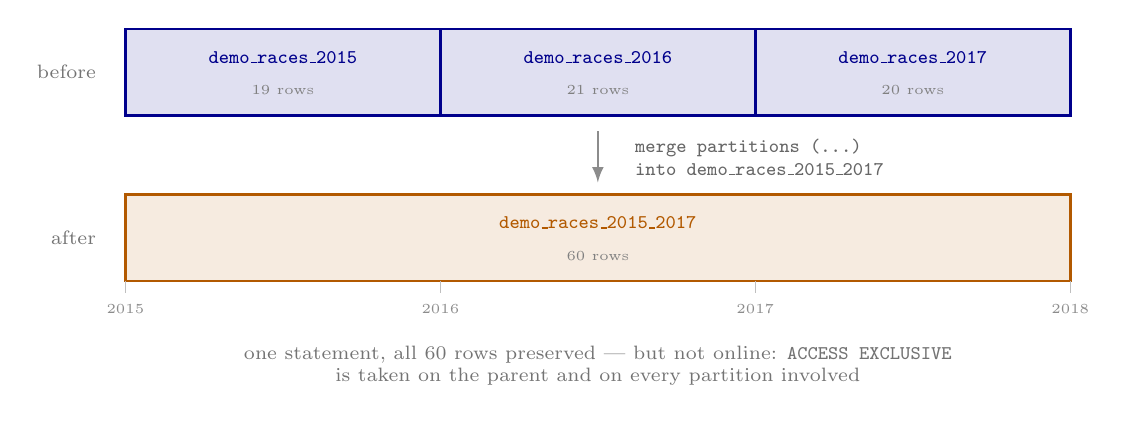
\begin{tikzpicture}[font=\small]

\colorlet{cPart}{blue!55!black}
\colorlet{cMerged}{orange!70!black}

%% Geometry: one season spans 4 units, 2015 -> x=0, 2018 -> x=12.
\def\xa{0}
\def\xb{4}
\def\xc{8}
\def\xd{12}

%% ---------- before: three partitions of one parent ----------
\node[anchor=east, font=\scriptsize, black!55] at (-0.25,3.15) {before};

\foreach \l/\r/\season/\rows in {0/4/2015/19, 4/8/2016/21, 8/12/2017/20} {
  \filldraw[cPart!12, draw=cPart, line width=0.9pt]
    (\l,2.6) rectangle (\r,3.7);
  \node[font=\scriptsize\ttfamily, cPart] at ({(\l+\r)/2},3.34)
    {demo\_races\_\season};
  \node[font=\tiny, black!50] at ({(\l+\r)/2},2.92) {\rows\ rows};
}

%% ---------- the statement ----------
\draw[-latex, black!45, line width=0.9pt] ({(\xa+\xd)/2},2.4) -- ({(\xa+\xd)/2},1.75);
\node[anchor=west, font=\ttfamily\scriptsize, black!60, align=left]
  at ({(\xa+\xd)/2+0.35},2.07) {merge partitions (...)\\into demo\_races\_2015\_2017};

%% ---------- after: one partition covering the whole range ----------
\node[anchor=east, font=\scriptsize, black!55] at (-0.25,1.05) {after};
\filldraw[cMerged!12, draw=cMerged, line width=0.9pt]
  (\xa,0.5) rectangle (\xd,1.6);
\node[font=\scriptsize\ttfamily, cMerged] at ({(\xa+\xd)/2},1.24)
  {demo\_races\_2015\_2017};
\node[font=\tiny, black!50] at ({(\xa+\xd)/2},0.82) {60 rows};

%% ---------- range bounds ----------
\foreach \x/\lbl in {0/2015, 4/2016, 8/2017, 12/2018} {
  \draw[black!25, thin] (\x,0.35) -- (\x,0.5);
  \node[font=\tiny, black!45, anchor=north] at (\x,0.32) {\lbl};
}

%% ---------- the caveat that matters operationally ----------
\node[anchor=north, font=\scriptsize, black!55, align=center]
  at ({(\xa+\xd)/2},-0.2)
  {one statement, all 60 rows preserved --- but not online: \texttt{ACCESS EXCLUSIVE}\\
   is taken on the parent and on every partition involved};

\end{tikzpicture}
\caption{\texttt{MERGE PARTITIONS} folds three range partitions into one.}
\end{figure}
